\contourlength{0.5pt}

\begin{figure}[h]
    \centering
    \adjustbox{valign=t}{
    \begin{minipage}{0.48\linewidth}
        {
            \centering
            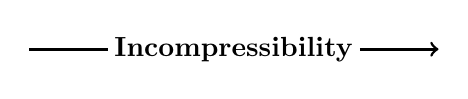
\begin{tikzpicture}
                \draw[-, line width=1pt] (.4,0) -- (1.4,0);
                \node at (3,0) {\textbf{Incompressibility}}; 
                \draw[->, line width=1pt] (4.6,0) -- (5.6,0);
            \end{tikzpicture} \\
        }
        \lfbox[
            border-width=2pt,
            padding-top=0pt,
            padding-bottom=0pt,
            padding-left=-2.5pt,
            padding-right=-2.5pt,
        ]{
            \begin{tikzpicture}
                \draw (0, 0) node[inner sep=0] {
                    \includegraphics*[width=0.25\linewidth]{overoptimization/neg-jpeg-ppo-hartebeest/0.jpg}
                };
                \node[text=black] at (-0.3, 0.6) {\scriptsize \contour{white}{\methodours{}}};
            \end{tikzpicture}
            \hspace{-0.7em}
            \includegraphics*[width=0.25\linewidth]{overoptimization/neg-jpeg-ppo-hartebeest/9.jpg}
            \hspace{-0.7em}
            \includegraphics*[width=0.25\linewidth]{overoptimization/neg-jpeg-ppo-hartebeest/49.jpg}
            \hspace{-0.7em}
            \includegraphics*[width=0.25\linewidth]{overoptimization/neg-jpeg-ppo-hartebeest/69.jpg}
        }
        \vspace{-0.5em} \\
        \lfbox[
            border-width=2pt,
            padding-top=0pt,
            padding-bottom=0pt,
            padding-left=-2.5pt,
            padding-right=-2.5pt,
        ]{
            \begin{tikzpicture}
                \draw (0, 0) node[inner sep=0] {
                    \includegraphics*[width=0.25\linewidth]{overoptimization/neg-jpeg-rwr-zebra/0.jpg}
                };
                \node[text=black] at (-0.4, -0.6) {\scriptsize \contour{white}{\methodrwr{}}};
            \end{tikzpicture}
            \hspace{-0.7em}
            \includegraphics*[width=0.25\linewidth]{overoptimization/neg-jpeg-rwr-zebra/1.jpg}
            \hspace{-0.7em}
            \includegraphics*[width=0.25\linewidth]{overoptimization/neg-jpeg-rwr-zebra/2.jpg}
            \hspace{-0.7em}
            \includegraphics*[width=0.25\linewidth]{overoptimization/neg-jpeg-rwr-zebra/3.jpg}
        }
    \end{minipage}
    }
    \adjustbox{valign=t}{
    \begin{minipage}{0.48\linewidth}
        {
            \centering
            
\begin{tikzpicture}
                \draw[-, line width=1pt, color=white] (0,0) -- (1,0);
                \node at (3,0) {\textbf{Counting Animals}}; 
                \draw[->, line width=1pt, color=white] (4.9,0) -- (5.9,0);
            \end{tikzpicture} \\
        }
        \lfbox[
            border-width=2pt,
            padding-top=0pt,
            padding-bottom=0pt,
            padding-left=-2.5pt,
            padding-right=-8.7pt,
        ]{
            \begin{minipage}{\linewidth}
                \includegraphics*[width=0.25\linewidth]{overoptimization/vlm-counting/six-lions.jpg}
                \hspace{-0.7em}
                \includegraphics*[width=0.25\linewidth]{overoptimization/vlm-counting/seven-birds.jpg}
                \hspace{-0.7em}
                \includegraphics*[width=0.25\linewidth]{overoptimization/vlm-counting/five-wolves.jpg}
                \hspace{-0.7em}
                \includegraphics*[width=0.25\linewidth]{overoptimization/vlm-counting/five-raccoons} \\
                \vspace{-1.2em} \\
                \includegraphics*[width=0.25\linewidth]{overoptimization/vlm-counting/eight-foxes.jpg}
                \hspace{-0.7em}
                \includegraphics*[width=0.25\linewidth]{overoptimization/vlm-counting/three-tigers.jpg}
                \hspace{-0.7em}
                \includegraphics*[width=0.25\linewidth]{overoptimization/vlm-counting/six-turtles.jpg}
                \hspace{-0.7em}
                \includegraphics*[width=0.25\linewidth]{overoptimization/vlm-counting/six-dogs.jpg}
            \end{minipage}
        }
    \end{minipage}
    }
    \caption{
        \textbf{(Reward model overoptimization)}
        Examples of RL overoptimizing reward functions.
        \textbf{(L)}~The diffusion model eventually loses all recognizable semantic content and produces noise when optimizing for incompressibility.
        \textbf{(R)} When optimized for prompts of the form ``$n$ \emph{animals}'', the diffusion model exploits the VLM with a typographic attack \citep{goh2021multimodal}, writing text that is interpreted as the specified number $n$ instead of generating the correct number of animals.
    }
    \label{fig:overoptimization}
\end{figure}